\documentclass{article}

\usepackage{pdfcomment}
\usepackage[margin=1in]{geometry}
\usepackage{xcolor}
\usepackage{graphicx}

\newcommand{\note}[2]{\pdfmargincomment[color=yellow,author=#1,open=true]{#2}}
\newcommand{\todo}[1]{\color{red}\textbf{TODO:}#1\color{black}}
\newcommand{\reprozip}[0]{ReproZip}

\title{Numerical error propagation in the HCP structural pre-processing pipelines}

\author{M. Ali Salari, Lalet Scaria, Gregory Kiar, Lindsay B. Lewis,
  Alan C. Evans, Tristan Glatard}

\begin{document}

\maketitle

\abstract{This paper is a reproducibility study of the work in~\cite{glasser2015multi}.}

\section{Introduction}

Operating systems are known to have an effect on the results produced
by neuroimaging pipelines~\cite{Gronenschild2012, Glatard2015},
presumably due to the creation, propagation and amplification of small
numerical errors across the pipelines.  Such errors highlight
numerical instability which is also likely to appear as a result of
other types of small perturbations such as acquisition and parametric
noise. However, the precise causes of
such instabilities and the path along which they propagate in the
pipelines are unclear.  We present a technique to identify the
processes in a pipeline that create numerical errors along the
execution, and we apply this technique to the HCP structural
pre-processing pipelines.


Groenschild \emph{et al.} first identified the effect of operating
systems on Freesurfer
results~\cite{Gronenschild2012}. In~\cite{10.3389/fninf.2015.00012} we
quantified this effect on some of the main neuroimaging pipelines
including several FSL pipelines, CIVET and Freesurfer. In this work we
aim at evaluating this effect on the work in~\cite{glasser2015multi}.
\todo{Link this to Lindsay's HBM 2017 poster and to Redolfi et al.}

The operating system is defined here as a consistent set of software
packages organized in a trusted repository.

The operating system is not the only part of the computational
environment that may hamper reproducibility. The work
in~\cite{diethelm2012limits} mentions reproducibility issues coming
from parallelization.

Notes:
\begin{itemize}
  \item Reproducibility has several other aspects, see, e.g.,
\url{https://medium.com/@lorenaabarba/barba-group-reproducibility-syllabus-e3757ee635cf#.ty3zmgd4k}
 \item James P Turner, speaker in INCF 2016 Track B, is looking at numerical stability on GPUs. And reproducibility.
 \item For an overview of variability accross analysis methods in fMRI, see \url{http://journal.frontiersin.org/article/10.3389/fnins.2012.00149/full}.
 \item For a general overview in fMRI, see \url{http://www.nature.com/nrn/journal/vaop/ncurrent/box/nrn.2016.167_BX3.html}
\end{itemize}

% There is a computational challenge
HCP preprocessing pipelines are both time-consuming and
computationally intensive which might even run for days, depending
upon the type and size of dataset.

Any
user who has access to this application can try to reproduce the
experiments since the data and the application are accessible within
the framework. However, one caveat is that, the neuroimaginng
pipelines might have different results due to differences in computing
platforms on which the images are getting processed
~\cite{10.3389/conf.fninf.2014.18.00076} therefore, the execution
results of the pipelines across different operating systems are
considered to find out the cause of the reproducibility issues using
an interposition techniques for the provenance capture.


\section{Materials and Methods}

\subsection{Data}

We randomly selected 10 subjects from the HCP data release
S500. \todo{ list the subjects.}

\subsection{HCP Minimal preprocessing Pipelines}

The Human Connectome Project (HCP)~\cite{Gla13} developed a set of
pipelines to help extraction of structural, functional or diffusion
MRI data across a large set of high resolution MR images. These
preprocessing pipelines create results that are available in standard
volume and combined surface and volume spaces which makes it easier
for researchers to compare the images across the neuroimaging
spectrum.

\paragraph{Structural Pipelines} The structural pre-processing consists of PreFreeSurfer, FreeSurfer and PostFreeSurfer. 
\paragraph{Functional Pipelines} Functional pre-processing consists of fMRIVolume and fMRISurface~\cite{FSL}. 
\paragraph{Diffusion Preprocessing pipeline} preparing...

\todo{Write a short summary of what the pipelines do.}

\subsection{Processing environment}

We executed the pipelines using Docker
containers to simplify the deployment of different operating
system versions on execution platforms. The Docker images were built for the HCP
 pre-processing pipelines v3.19.0 (PreFreeSurfer and
FreeSurfer)~\cite{Glasser2013} in CentOS 6.8 and CentOS 7.2. Docker images are available on DockerHub for reuse \url{https://hub.docker.com/r/bigdatalabteam/hcp-prefreesurfer/}. We
collected the provenance trace (tree of executed processes and files
accessed in read or write mode) for each type of subjects using system-call
interception as provided by the \reprozip tool~\cite{Chirigati2016}.



To support the computational challenge, we used the Canadian Brain
Imaging Research Platform (CBRAIN)~\cite{cbrain} to manage the
containers and data. CBRAIN is a Web platform developed at the
Montreal Neurological Institute (MNI) to tackle the computational
challenges faced by neuroimaging researchers.  Applications can be
ported to CBRAIN using the Docker and Singularity container
technologies through the Boutiques framework~\cite{boutiques}. Our
CBRAIN HCP plugins are publicly available at \url{https://github.com/glatard/cbrain-plugins-hcp} for
installation and re-use in CBRAIN instances.

We processed subjects twice in every condition to identify possible \emph{intra-condition} errors coming from the use of pseudo-random numbers or other external
factors. 

To further ensure that the observed errors are caused by operating system
updates (\emph{inter-os differences}) and not by other factors, we
implemented the following sanity checks:
\begin{itemize}
\item The file checksums of every
subject are computed before and after processing to detect potential corruption during file transfers and other manipulations.
\item The checksum of the Docker container images is recorded with
  every execution to identify any unintentional package update. In
  addition, the list of packages with versions is printed by every
  task and checked for consistency.
\item Hardware information is captured to make sure that errors are
  not coming from different CPU architectures.
\item Every task is executed on its own copy of the data to ensure
  that input data is not modified by the pipeline. 
\end{itemize}

\todo{Check ~\cite{DBLP:journals/fini/DasGRSPMSRSKMKR17}}

\subsection{Measuring differences}



We computed a file difference matrix between files produced for every
subject in every operating system based on MD5 checksums~\cite{md5}
(\url{https://tools.ietf.org/html/rfc1321}) as
in~\cite{Scaria2017}. MD5 is suitable to identify incidental file
differences, although it is not cryptographically secure. Files
produced only in some subjects or in some operating systems were left out.

We quantified the error in the image files using the Dice coefficient and normalized root mean square error (NRMSE) computed as follows:
\begin{center}
\begin{equation}
RMSE = {\sqrt {\frac{1} {n}{\sum\limits_{t = 1}^n {(\hat{y}_{t} - {y}_{t} } })^{2} } }
\end{equation}
\end{center}

\begin{center}
\begin{equation}
NRMSE = {\frac{RMSE} {y_{max} - y_{min}}}
\end{equation}
\end{center}

\subsection{Pipeline analysis: Characterizing differences}

Once differences between conditions are quantified, we automatically
identify the steps in the pipeline responsible for such differences.
We use the \reprozip tool~\cite{reprozip} to record: (1) the tree of
processes executed by the pipeline and (2) the list of files read and
written by each process. This information is collected by system call
interceptions, through the \texttt{ptrace} as a UNIX base system call, and stored in a \texttt{SQLite}
database. The database stores information on all the processes which
are created by the \texttt{clone()} in Linux or \texttt{fork()} in UNIX-like
operating system calls. It also records the files opened by each process (in read, write or execution mode), including the final and
temporary files.

We reconstruct the tree of processes starting from the first process
created by the pipeline and defining its child processes as the ones
that were created through \texttt{clone()} or \texttt{fork()}. We
create a process graph from this tree by adding edges corresponding to
file dependencies between processes. A file dependency is defined
between processes A and B if a file written by A is read by
B. Figure~\ref{fig:graph-example} shows an example of a process graph
constructed at this stage.

\begin{figure}
%  \includegraphics{brain\_classification}
  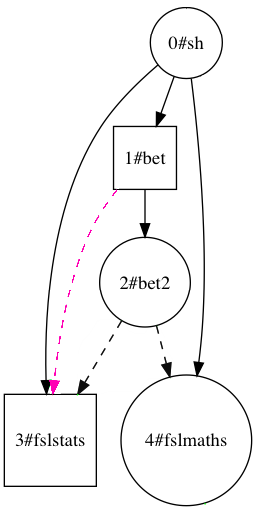
\includegraphics[scale=0.3]{images/simple_graph}
  \caption{Process graph constructed from an example brain extraction script.}
  \label{fig:graph-example}
\end{figure}

A different process graph may be produced for every subject in every
execution condition. Among our dataset, we identified 4 types of
subjects with different numbers of T1w and T2w images. We verified
that the process graphs were identical for all subjects of the same
type, for all execution conditions. The remainder of the analysis is
done separately for each subject type.

Cycles may be present in the process graph in case a file was written
by more than one process.  We remove the cycles in the process graph
by removing file edges between processes A and B when A's process
creation timestamp is posterior to B's or when A=B.

\todo{Start from here}
\paragraph{} In the next step, we classify the processes into three categories considering to the obtained process tree 
and the error matrix file. First, processes that read file(s) without error but write different file(s) create error in 
the pipeline. The second group of the processes are those which remove errors in pipeline, read file(s) with error and
 write “nothing or” file(s) without error. Most of the processes are in the third category beyond any fault which
 read and write file(s) without error. The processes in each category may read or write temporary file(s) that implies 
the uncertainty of the process.
\paragraph{} Pipeline is conducted of a bunch of processes sequentially, setting a modification step after classification
 of processes iteratively enables us to control the propagation of errors in the pipeline correctly. In each iteration
 we detect all the processes which are create error in the pipeline and then by fixing those processes artificially, 
we’ll find the other processes in the pipeline that introduce an error. This procedure will be terminated by fixing all the processes. 
To fix the processes that create error, we replace their dependency files with error by the same file copy from the results 
obtained in the other operating system. In this way, we were able to pinpoint the origin of the errors measured in the pipeline.

\todo{Check that} We also recorded the provenance trace of the execution using \reprozip. \reprozip identifies all the
processes and associated parameters that wrote the files having
differences.  These details about various processes is helpful in
debugging the pipelines. This information helps in recreating the
processing step by step and also to identify the processes that
creates the differences.


\section{Results}

Show lists of packages used with version. Focus on important
differences (e.g.: python interpreter, gcc if relevant) and explain
why these packages are important.

Show results of the comparison.

\subsection{Inter-OS differences}


\paragraph{Binary differences}


Among the 117 data files produced by PreFreeSurfer, 21 did not have any error for any subject, 92 had errors 
for all subjects and 4 had errors for 3 subjects only. 

In a previous study~\cite{Scaria2017}, we showed that
pre-processing pipelines of the Human Connectome
Project~\cite{Glasser2013} were sensitive to operating system
variation (see Figure \ref{fig:1}).
\begin{figure}
%  \includegraphics{brain\_classification}
  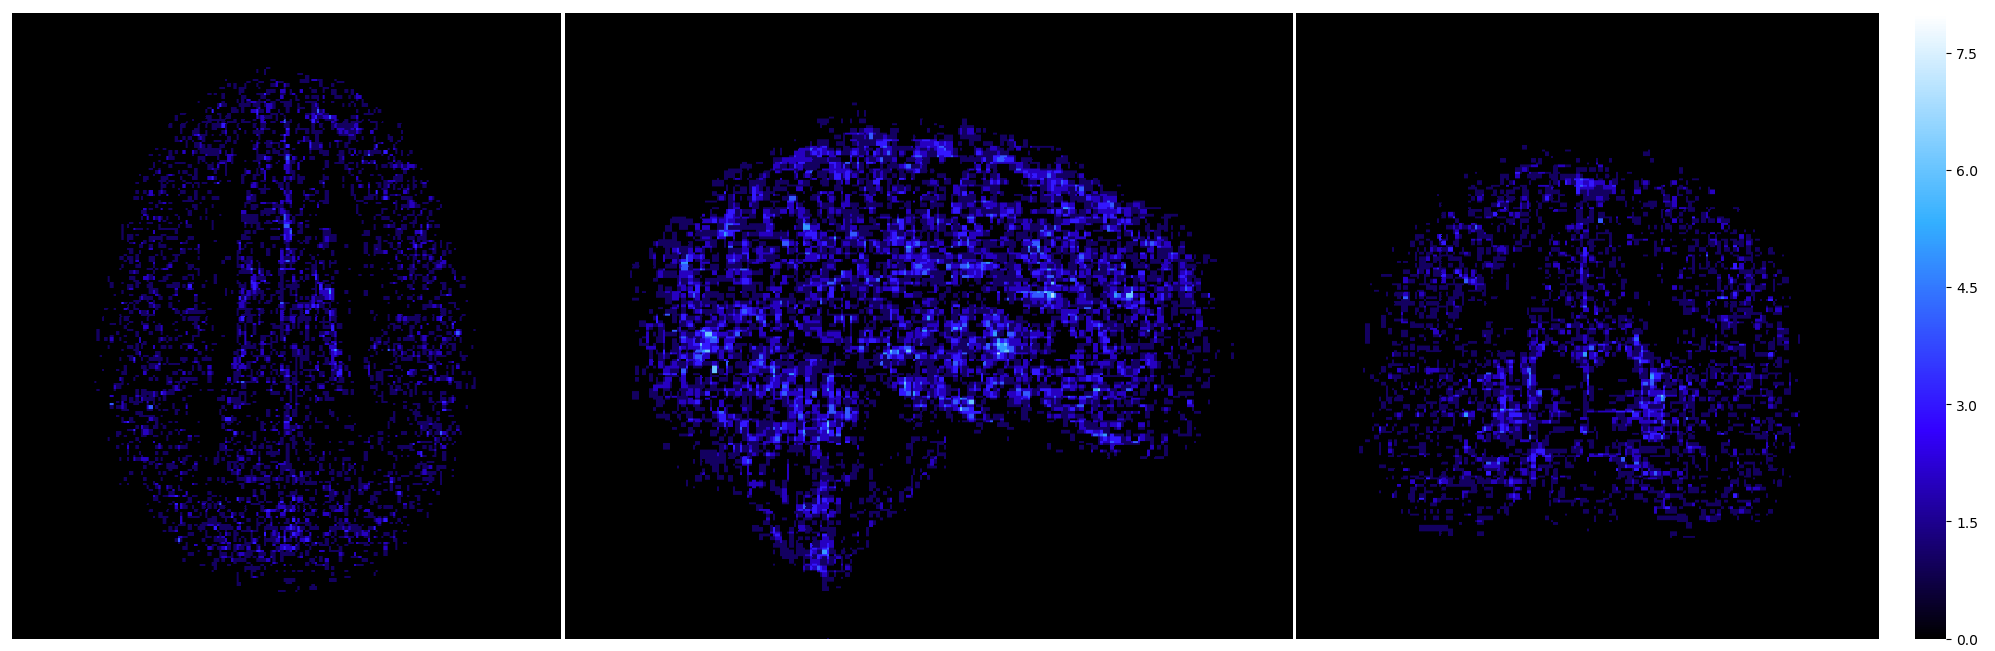
\includegraphics[width=0.5\textwidth, height=6cm]{images/brain_classification.png}
  \caption{Tissue classification produced by the HCP pre-processing
    pipelines on subject 105216 (CentOS 6 vs CentOS 7).}
  \label{fig:1}
\end{figure}

\paragraph{}
Two types of differences can occur in the subjects due to the differences in the operating systems. 
One is inter-OS difference caused by the operating system library updates and the other type,
 intra-OS differences occurs as a result of the pseudo-random processes used in the pipelines.
 An example of a pseudo-random process function is, a random number generator that would get initialized 
using a seed state. the proposed method can be used to identify both kind of differences. 
The files that are common to all the subjects only are taken into consideration for comparison. The first step
 is identification of files with differences in their checksums. This is identified using the checksums that are
 recorded after the processing. Intra-OS differences are identified using the run-number added as the suffix for
 the conditions. For example, the two batches of subjects processed under the same condition (CentOS6) are stored 
as run-1 and run-2. The files belonging to the subjects stored under the above mentioned conditions are treated as intra-OS runs.



\subsection{Pipeline analysis}

Figure \ref{fig:2} shows the annotated provenance graph of the
PreFreeSurfer pipeline executed on CentOS6 and CentOS7.  Processes
that created errors are shown in red, processes that removed errors
are in blue, and other processes are in green.  Squares denote
processes for which the classification is uncertain, due to temporary
files that were removed during the execution. Black edges link
sub-processes to their parents while dashed edges denote file
dependencies between processes (green edges: files with no errors; red
edges: files with errors; yellow edges: temporary files).  The
processes that introduce errors in PreFreeSurfer are: linear
registration with “\emph{FLIRT}” (8 occurrences, in ACPC Alignment,
BrainExtraction, DistortionCorrection, AtlasRegistration), non-linear
registration with “\emph{FNIRT}” (3 occurrences, in BrainExtraction
and AltasRegistration), image warping with “\emph{new\_invwarp}” (3
occurrences, in BrainExtraction and AtlasRegistration).  In addition,
errors were observed in image mean and standard-deviation computations
with “\emph{fslstats}” (3 occurrences in BiasFieldCorrection), and in
masked image extrapolation with “\emph{fslmaths}” (1 occurrence, in
BiasFieldCorrection).  Besides, transformation format conversion with
“\emph{convertwarp}” (2 occurrences, in DistortionCorrection) was able
to remove errors.

\todo{Check if a given file is written by only one process (add a safeguard in your code).}

\begin{figure}
  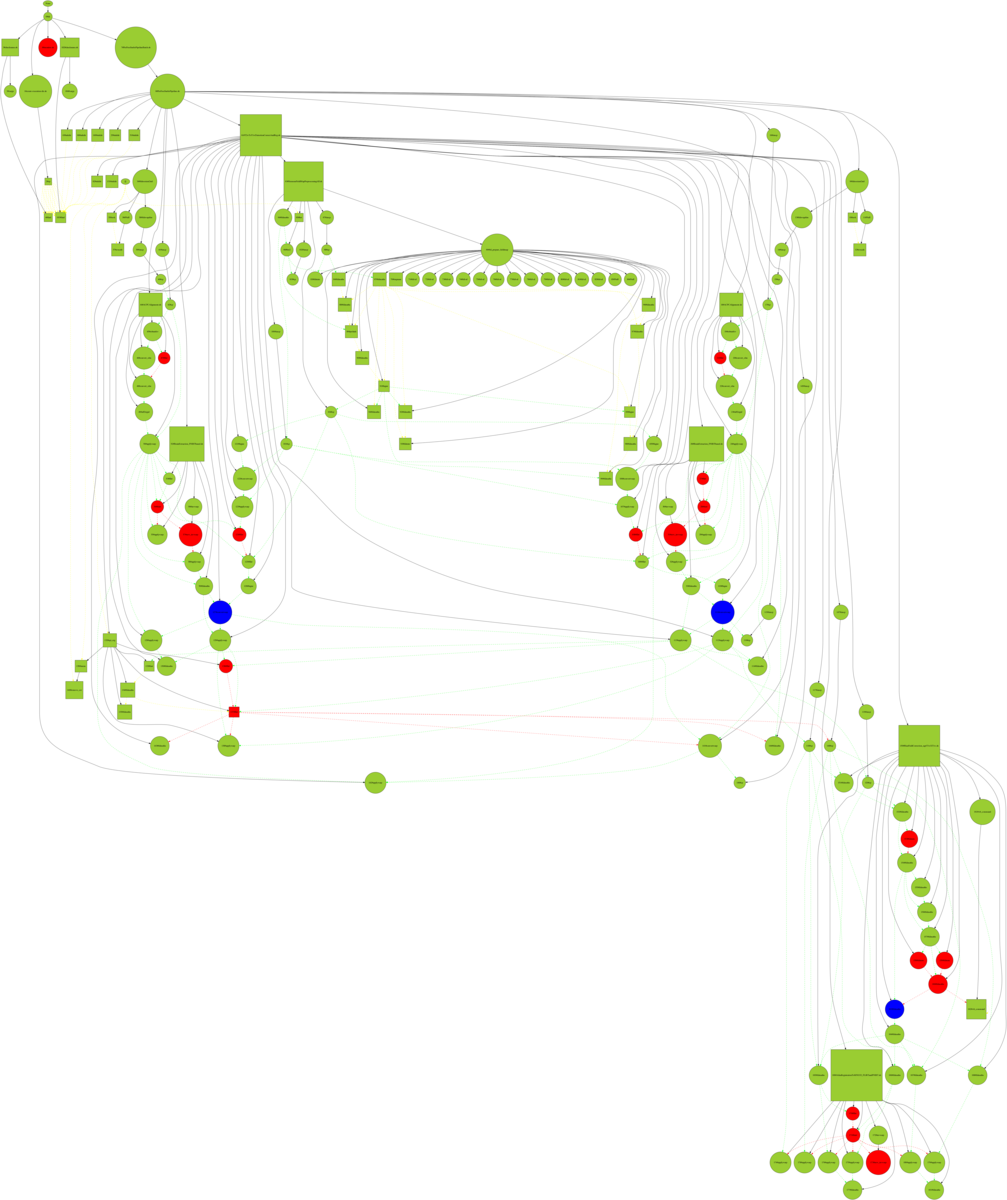
\includegraphics[width=\linewidth]{images/graph}
  \caption{An annotated provenance graph from the PreFreesurfer pipeline. Processes that created errors are in red. 
Full-resolution image available at \url{https://drive.google.com/open?id=174yyn8SuVOUcK5aRVw0bagjDanLD0FLt}.}
  \label{fig:2}
\end{figure}

\section{Discussion}

Discuss the results.

Mention that this was only possible because the unprocessed data was shared in the first place.

DICOM to Nifti conversion was out of scope and may introduce other issues.

\section{Conclusion}

Conclude and highlight future work.

The numerical instability in the PreFreesurfer HCP pipeline arises mainly from linear and non-linear registration processes 
implemented in FSL FLIRT and FNIRT. These processes need to be reviewed to understand and correct the cause of instabilities. 
In this correction process, accuracy has to be considered in addition to stability. Our technique is able to 
characterize the stability of a pipeline’s components automatically, but it also suffers from limitations as it cannot deal with: 
(1) results that are not written to disk (values processed in memory); (2) temporary files (3) files that are written by more than one process.


\section{Acknowledgments}

CBRAIN team. Compute Canada(Calcul Quebec).

\bibliographystyle{plain}
\bibliography{biblio}

\end{document}
